\documentclass[12pt]{article}
\usepackage[papersize={8cm,12cm},margin={.5cm,.5cm}]{geometry}
\usepackage{common}
\usepackage{amssymb}
\begin{document}
\begin{problem}
  \item[8.] 圖(四)中有一直圓柱,其底面半徑為 $1$ 公分,柱高為 $3$ 公分。若此圓柱的體積為 $V$ 立方公分,則 $V$ 的值是多少?
  \begin{figure}[ht]
    \centering
    \vspace*{-1ex}
    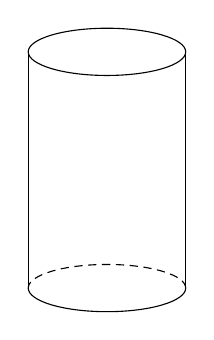
\begin{tikzpicture}
      \draw (0,3) ellipse (1 and .3);
      \draw (-1,0) arc (180:360:1 and .3);
      \draw[densely dashed] (1,0) arc (0:180:1 and .3);
      \draw (-1,0) -- (-1,3);
      \draw (1,0) -- (1,3);
    \end{tikzpicture}
    \vspace*{-1ex}
    \caption*{圖(四)}
    \vspace*{-2ex}
  \end{figure}
  \begin{choices}
    \item $\pi$
    \item $2\pi$
    \item $3\pi$
    \item $6\pi$
  \end{choices}
\end{problem}
\end{document}
